\documentclass[a4paper,kul]{kulakarticle} %options: kul or kulak (default)

\usepackage[utf8]{inputenc}
\usepackage[dutch]{babel}
\usepackage{float}
\usepackage{subcaption}

\date{Academiejaar 2019 -- 2020}
\address{
  Faculteit Industriële Ingenieurswetenschappen \\
  Systeemontwerp met HDL \\
  S. Verslype}
\title{Verslag spectrogram}
\author{Robin Nollet, Sebastian Vantomme, Ine Vanderhaeghe}


\begin{document}
	
\maketitle
	
\begin{center}
	\centering
	\vspace*{\fill}
	\huge
	\textbf{Verslag: bouwen van een spectrogram op een FPGA met behulp van de VHDL-taal}
	\vspace*{\fill}
\end{center}
	
\newpage
	
\tableofcontents

\newpage

\section{Probleemstelling: een audiospectrogram}

Doorheen het semester hebben we ons met ons groepje bezig gehouden met het bouwen van een audiospectrogram.

\subsection{Wat is een spectrogram?}

Het kan handig zijn om snel de frequentieinhoud van een signaal te zien, naar analyse toe. Gezien een signaal ook vaak veranderlijk is in de tijd, kan ook de frequentieinhoud veranderen in functie van de tijd. Er bestaat een methode om de frequentieinhoud van een signaal weer te geven in functie van de tijd. Dit heet een \textit{Spectrogram}. Een spectrogram kan goed samengevat worden volgens de volgende definitie: het is een visuele representatie van de energie in elke frequentie uitgezet in de tijd. Een spectrogram heeft verschillende toepassingen. Enkele voorbeelden hiervan is bv. in de audio, of in de analyse van licht. Dit project focust specifiek op het analyseren van audiosignalen, hoorbaar voor het menselijk oor. Hiervoor nemen we standaard een range van $20Hz$ tot $20kHz$. In de audiowereld worden deze frequenties vaak de \textit{pitch} genoemd van het signaal. 


Mogelijke toepassingen van een spectrogram die hoorbare audiosignalen worden hieronder opgesomt:
\begin{itemize}
	\item analyse van Muziek(-instrumenten)
	\item analyse van Spraak
	\item analyse van Dierengeluiden
	\item analyse van RF modulatietechnieken
\end{itemize}

\subsection{Hoe wordt een spectrogram voorgesteld?}

De grafische voorstelling van een spectrogram zou eigenlijk in 3 dimensies moeten gegeven worden. Dit is echter wat lastig om dan op één oogopslag informatie te kunnen uit aflezen. Daarom worden in de literatuur vaak de volgende afspraken gevolgd:
\begin{itemize}
	\item De tijd wordt op de horizontale as uitgezet;
	\item De frequentie wordt op de verticale as uitgezet;
	\item De sterkte van de frequentie wordt vaak weergegeven met behulp van kleurintensiteit of een kleurgradiënt.
\end{itemize}
In figuur \ref{fig:typischegrafischevoorstellingspectrogram} is een typische grafische voorstelling gegeven.

\begin{figure}[H]
	\centering
	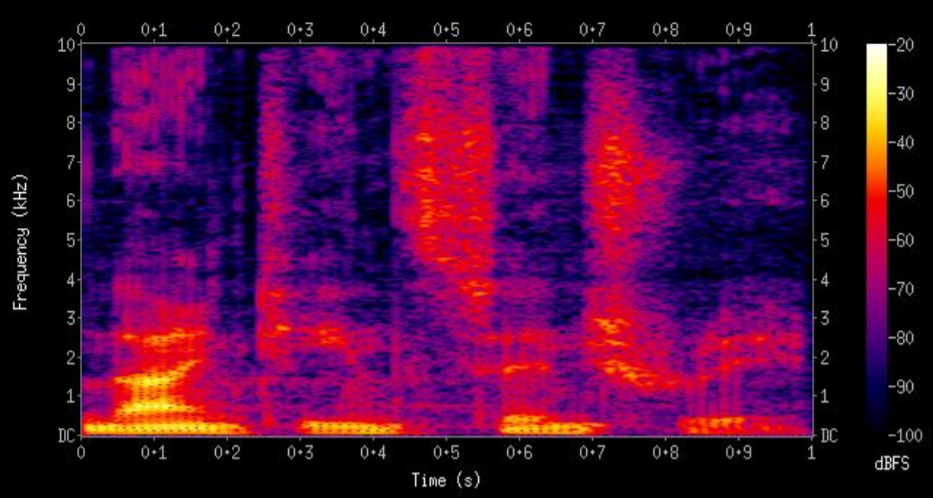
\includegraphics[width=0.7\linewidth]{typischeGrafischeVoorstellingSpectrogram.png}
	\caption{Een typische grafische voorstelling van een spectrogram}
	\label{fig:typischegrafischevoorstellingspectrogram}
\end{figure}

\subsection{Gebruikte methoden om een spectrogram te implementeren}

In de literatuur kunnen 2 veelgebruikte methoden voor de implementatie van een Spectrogram gevonden worden.
\begin{enumerate}
	\item Met behulp van de FFT: van het ingenomen signaal wordt de \textit{Fast Fourier Transform (FFT)} genomen, wat een versnelde versie is van de \textit{Discrete Fourier Transform (DFT)}. Dit toont de frequentieinhoud van het signaal. Een belangrijke eigenschap van deze transformatie is dat ze een discrete ingang (de audio) en een discrete uitgang (de frequentieinhoud van dit signaal) heeft. 
	\item Met behulp van een filterbank: hier wordt een reeks banddoorlaatfilters geïmplementeerd, die allemaal op hetzelfde signaal werken. Door na iedere filter dan te gaan kijken wat de energie van het signaal is, kan dit als een maat gebruikt worden voor de frequentieinhoud van ons ingangssignaal.
\end{enumerate}

Naar implementatie toe heeft men dan een keuze, dit hangt af welke resolutie men wilt in de frequentie. Wil men een grote resolutie in de frequentie, gaat men eerder kiezen voor de aanpak met de FFT. Als men met een lage frequentieresolutie zich tevreden kan nemen, wordt er vaak geopteerd voor de implementatie met die meerdere filters.\\
Wij hebben hier gekozen voor de implementatie met een FFT, omdat deze een stuk flexibeler is in implementatie.


\subsection{Afwerkingsgraad}

Onze opdracht bestaat er uit om zelf een real-time spectrogram te maken van een audiosignaal dat aangeboden wordt door een FPGA. Dit spectrogram moet gevisualiseerd worden op een extern scherm via VGA of HDMI. \\

Als eerste moet er dus een analoog audiosignaal kunnen binnengelezen worden via de audiocodec chip. Deze zorgt zelf voor de digitalisatie van het signaal en geeft dit door aan de FPGA. Er moet dus communicatie mogelijk zijn tussen de codec chip en de FPGA. \\
Daarna moet het spectrum bepaald kunnen worden. Er worden een aantal samples genomen op het gedigitaliseerde audiosignaal. Daarop wordt een FFT uitgevoerd. Hierbij kan gewerkt worden met aansluitende of overlappende blokken van de samples. Als met overlapping gewerkt wordt zou de resolutie fijner zijn, maar het zou ook complexer zijn. \\
Ten laatste moet de verzamelde data na de FFT op een 2D map komen die het spectrogram voorsteld. Eens het volledige scherm gevuld is, moet de oudste meting verwijderd worden en schuift het spectrogram een tijdseenheid op via een FIFO. \\

In het volledige systeem moet rekening gehouden worden met de timing en mogelijke asynchrone signalen. \\
Er zal tijdens de evaluatie van het project met verschillende testsignalen gecontroleerd worden als het project juist ontworpen is. Voorbeelden van testsignalen zijn FM modulatie, frequentie sweep, blokgolf, DTMF signalen, ... \\
\\ Er zijn enkele minimum vereisten in dit project:
\begin{itemize}
	\item Er wordt gewerkt met een FPGA bord naar keuze (Zedboard, Zybo, PYNQ, ...)
	\item Interface met audiocodec chip
	\item Real-time FFT op audio input
	\begin{itemize}
		\item 1 kanaal (mono)
		\item Aansluitende blokken van \textit{N} samples
	\end{itemize}
	\item Opstellen en updaten van spectrogram
	\item VGA/HDMI interface logica
	\item Beschikbaar stellen van spectrogram op een extern beeldscherm
\end{itemize}
Daarnaast zijn nog enkele mogelijkheden tot uitbreiding:
\begin{itemize}
	\item Stereo spectrogram
	\item FFT op overlappende tijdssignalen
	\item 3D spectrogram
	\begin{itemize}
		\item Amplitude als kleurintensiteit
	\end{itemize}
	\item Full HD
	\item Audio loopback
	\begin{itemize}
		\item Signaal terug naar buiten via line-out of headphone
	\end{itemize}
\end{itemize}

\section{Oplossingsstructuur}
Voor dergelijke probleemstelling is de eerste stap om een \textit{pipeline} op te stellen, een stappenplan van wat er met de data moet gebeuren van input tot aan output. Bij deze opdracht hebben we de pipeline toegepast gevonden in figuur \ref{fig:toegepastePipeline}.

\begin{figure}[H]
	\centering
	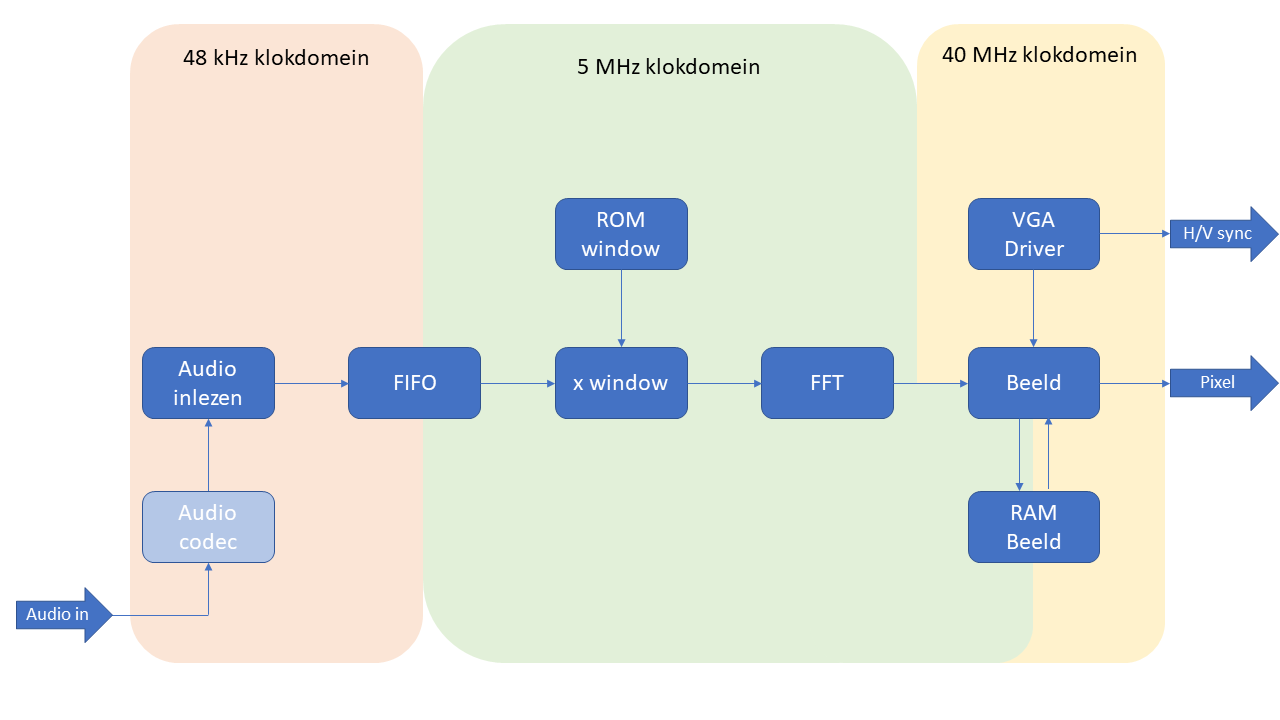
\includegraphics[width=0.7\linewidth]{Pipeline.png}
	\caption{toegepaste pipeline}
	\label{fig:toegepastePipeline}
\end{figure}

Zoals te zien valt op de figuur is het werk grotendeels op te splitsen in 3 grote delen, namelijk aan de hand van het klokdomein. Er hoeft dan gewoon via een dual-port-RAM een overschakeling te worden gemaakt tussen deze verschillende klokdomeinen. We hebben het werk opgesplitst in de volgende delen:

\begin{enumerate}
	\item Audio inlezen. Kort samengevat is dit het inlezen van de audio via de audiocodec en stockeren in de FIFO.
	\item Fourier nemen. Dit is de data uit de FIFO halen, er een window op toepassen en er daarna de fouriertransformatie op loslaten. De output van de FFT wordt dan doorgegeven aan Beeld.
	\item Grafisch weergeven. Hier wordt de data gegeven van de FFT opgeslagen in een RAM, die dan ook wordt uitgelezen aan een andere kloksnelheid. Zo wordt de data visueel op het scherm gerepresenteerd.
\end{enumerate}

\subsection{Audio inlezen}

Om de audio binnen te lezen, zijn er 2 belangrijke bestanden: \textit{adau1761} en \textit{audio\_if}. Deze bestanden lezen de data binnen en genereren daar de juiste clock signalen voor. In het top level wordt daar dan een audio loopback van gemaakt om de data die binnengelezen werd ook weer naar buiten te sturen. De data die binnengelezen werd wordt ook naar een FIFO gestuurd, zodat deze op de juiste momenten binnengelezen kan worden in de fft controller.

\subsection{Fourier nemen}
%SEBA

\subsection{Grafisch weergeven}
% ROBIN

\section{Implementatie}
%Algemeen overzicht

\subsection{Audio inlezen}

Er kan gebruik gemaakt worden van de audiocodec die aanwezig is op het Zedboard. Dit is de \textit{adau1761}. Hiervoor moest een driver geschreven worden. Voor ons project hebben we een driver kunnen gebruiken die we gekregen hadden van Dhr. Verslype. Deze driver krijgt zowel serieel als parallelle data binnen. De samples van het linker en rechter kanaal zijn 24 bit breed. Deze worden verwerkt in de driver en er wordt een linker en rechter output gegenereerd die 24 bit breed zijn en een seriële data output. \newline

Daarnaast moest een interface geschreven worden die de clock genereerd en de data die de driver binnenleest op een juiste manier door geeft naar het top level. Ook hier hebben we gebruik gemaakt van een interface die we gekregen hadden van Dhr. Verslype. Deze interface heeft een kloksignaal nodig van 100 MHz en 12,288 MHz. Deze genereren 3 nieuwe kloksignalen: de \textit{master clock}, de \textit{digital audio bit clock} en de \textit{digital audio left-right clock}. Deze worden gebruikt in de adau1761 codec. \newline

De configuratie van de audio interface werkt met het $I^2C$ protocol, het doorgeven van audio data gebeurt via het $I^2S$ protocol.\newline

In het top level wordt daarna een audio loopback gemaakt. De data wordt ook doorgegeven aan een FIFO memory, zodat deze uitgelezen kan worden door de fft controller. De data wordt serieel doorgegeven, eerst moet deze dus geparallelliseerd worden en per 24 bits opgeslagen worden in de memory. Het memory is 2048 waarden groot, dus wanneer deze vol is wordt een flag hoog gezet zodat de fft controller weet dat alle waarden die in de memory staan geldig zijn. 

\subsection{Fourier nemen}
% SEBA

\subsection{Grafisch weergeven}
% ROBIN

\section{Besluit}
% INE

Afsluitende tekst.

\end{document}
